\section{Core architecture}
Xilinx has introduced the AXI4-Stream interface \cite{ug761} for the Virtex-7 PCIe core, this is a simplified version of the ARM AMBA AXI bus \cite{arm}  which doesn't contain any address lines. Instead the Address and other information are supplied in the header of each PCIe package. Figure~\ref{fig:pcie_core_structure} shows the structure of the PCIe DMA Core design. The DMA core is divided in two parts:
\begin{enumerate}
\item DMA Control \\This is the entity in which the descriptors are parsed and fed to the engine, and where the status register of every descriptor can be read back through PCIe. DMA control contains a register map, with addresses to the descriptors, status registers and external registers for the user application.
\item DMA Read Write \\This entity contains two processes:
\begin{itemize}
\item Add Header\\In the first process the descriptors are read and a header is created according to the descriptor. If the descriptor is a write descriptor, the payload data is read from the FIFO and added after the header.
\item Strip Header\\In the second process the header of the received data is checked against the tag of the request, and the payload is shifted into the FIFO.
\end{itemize}
Both processes can fire an MSI-X type interrupt through the interrupt controller when the processing of a descriptor is completed.
\end{enumerate}
\begin{figure}[H]
\centering
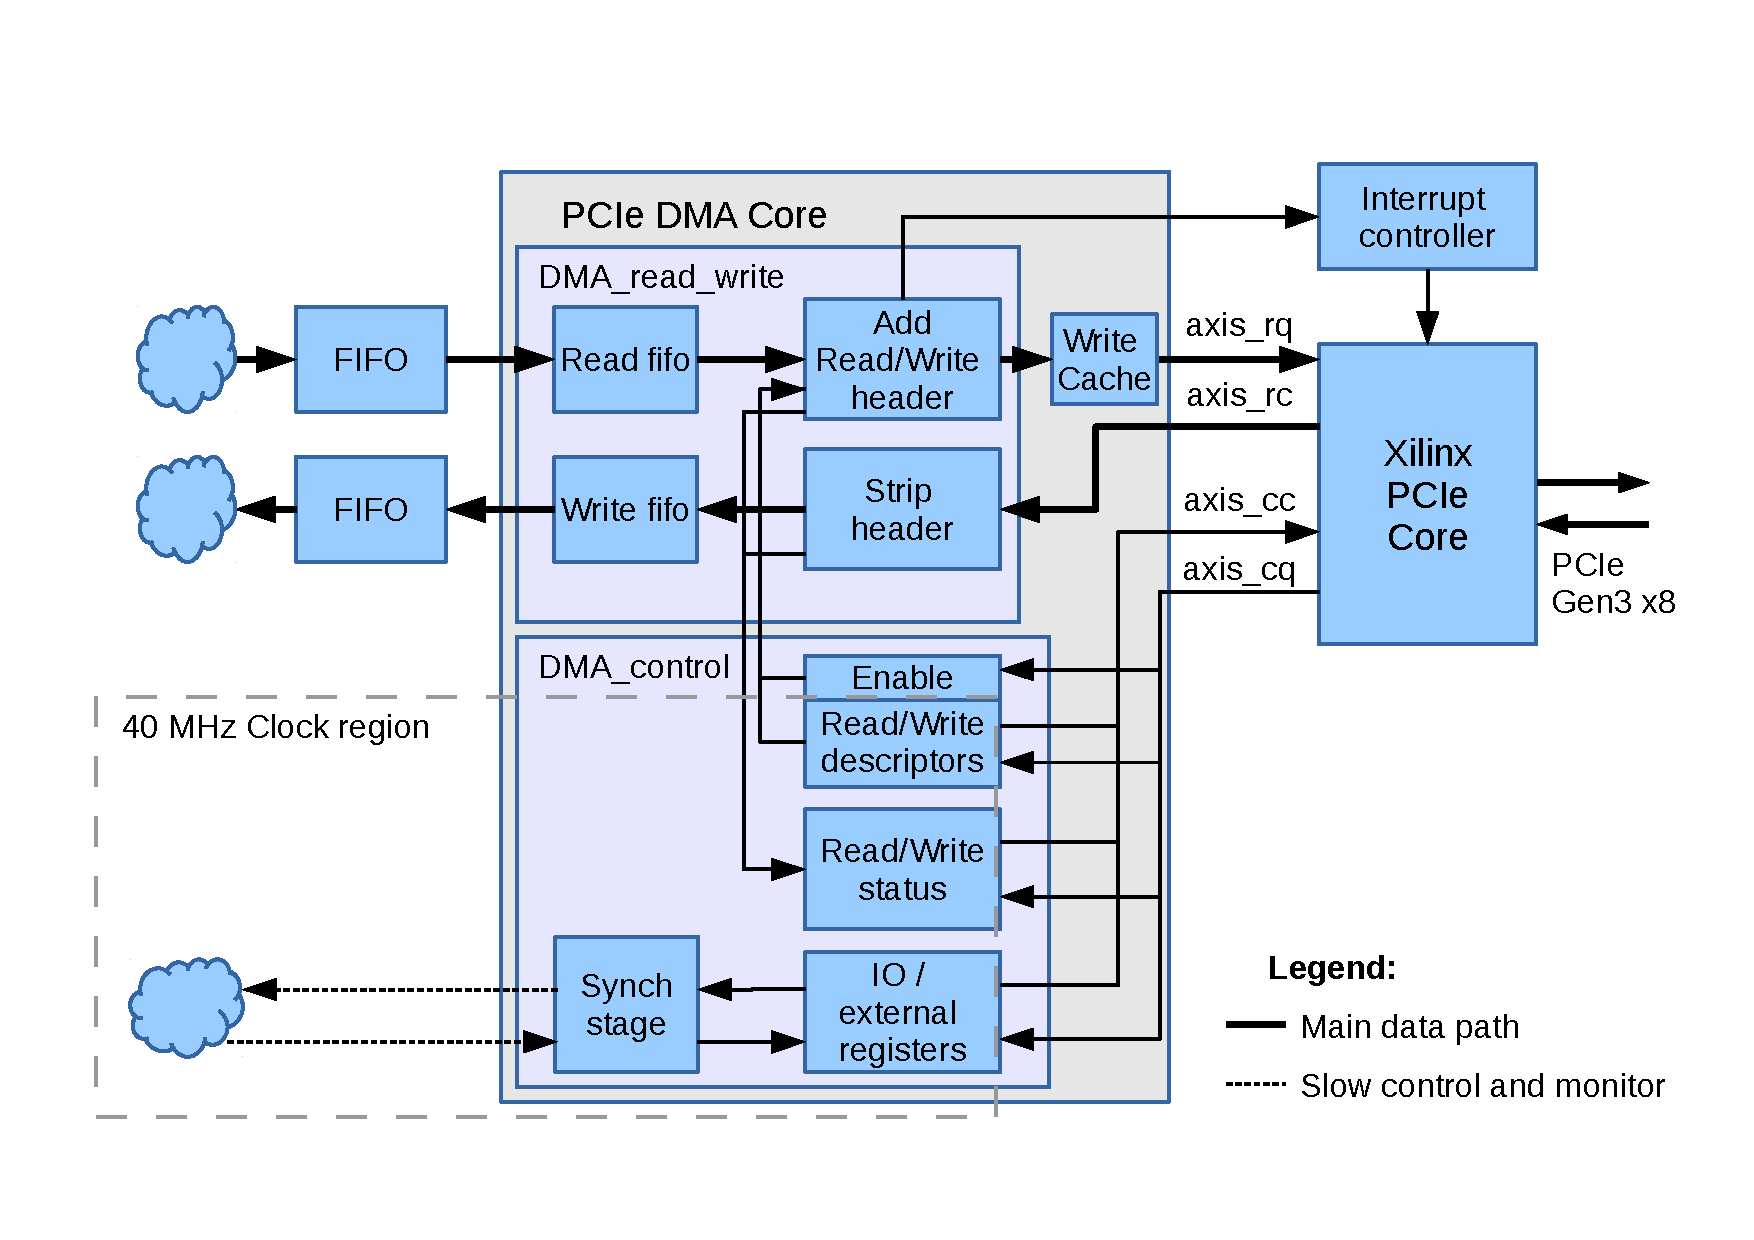
\includegraphics[trim=0mm 0cm 0mm 1cm,width=0.75\textwidth, page=1]{pictures/dma_core_structure.pdf}
\caption{Structure of the PCIe DMA core}
\label{fig:pcie_core_structure}
\end{figure}
Figure~\ref{fig:pcie_core_structure} also shows the sync stage for the IO and external registers. The user space registers are synchronized to a slower clock (e.g. 40 MHz) in order to relax timing closure of the design. To make sure no glitches or latch-up will occur, the synchronization stage does not update during a write cycle of the DMA Control process.
\begin{figure}[H]
\centering
\includegraphics[trim=0mm 2cm 0mm 1cm, width=0.75\textwidth, page=2]{pictures/dma_core_structure.pdf}
\caption{Flow of a Register / Descriptor Read or Write process}
\label{fig:flow_dma_control}
\end{figure}
The DMA Control process always responds to a request with a certain $req\_type$ from the PC. It does only respond to IO and Memory reads and writes, for all other request types it will send an unknown request reply. If the data in the payload contains more than 128 bits, the process will send a "completion abort" reply and go back to idle state. The maximum register size has been set to 128 bits because this is a convenient maximum register size; it is also the maximum payload that fits in one 250 MHz clock cycle of the AXI4-Stream interface.

\begin{figure}[H]
\centering
\includegraphics[trim=0mm 1cm 0mm 0cm, width=0.75\textwidth, page=3]{pictures/dma_core_structure.pdf}
\caption{Flow of the DMA Write, or Read request process}
\label{fig:flowdma_write}
\end{figure}
The DMA write process reads the current descriptor and requests a read or write to the PC memory. For a write it also initiates a FIFO read and adds the data into the payload of the PCIe packet. When initiating a read request, this process will additionally copy the current $tag$ into an array of tags which will be used in the DMA read process in order to check a matching reply. 
\begin{figure}[H]
\centering
\includegraphics[trim=0mm 3cm 0mm 1cm, width=0.75\textwidth, page=4]{pictures/dma_core_structure.pdf}
\caption{Flow of the DMA Read process}
\label{fig:flow_dma_read}
\end{figure}
The DMA read process checks the header for a valid tag, created by the DMA Write process, if this header and tag is valid, the data will be pushed into the FIFO.
\begin{figure}[H]
\centering
\includegraphics[trim=0mm 3cm 0mm 1cm, width=0.75\textwidth, page=5]{pictures/dma_core_structure.pdf}
\caption{Flow of the Backup cache process}
\label{fig:flow_dma_cache}
\end{figure}
In case the PC (or PCIe master) sends back-pressure by deasserting the AXI4 $tready$ signal in the $axis\_rq$ bus during a Transaction Layer Packet (TLP) transfer, it has been observed that the content of the TLP may get lost, even though the TLP will apparently complete successfully. Therefore the entity DMA\_Cache has been introduced, it will record all TLPs and play it back whenever back pressure occurs.

\newpage